%%%%
\section{Fluorescência de Raios X}

Para determinação e quantificação das composição química (número atômico $ 10 < Z < 82$)
das amostras foi utilizada a técnica não-destrutiva de \textit{Fluorescência de Raios X}.
\textit{Fluorescência de Raios X} é um método analítico quali-quantitativo, 
multielementar, que mede os raios-X característicos emitidos dos átomos da amostra, 
depois de também serem excitados por Raios X. Não exige pré-tratamento químico
das amostras e permite análise simultânea dos elementos químicos.

Existem 3 Tipos de fluorescências de raios X: dispersão em energia,
dispersão por comprimento de onda e reflexão total.
O usado nessa pesquisa foi o 
\textit{Fluorescência de Raios X por dispersão em energia} \cite{jenkins1988}.

A figura \ref{fig:shimadzu_atomo} ilustra classicamente o que ocorre com
o átomo ao ser excitado.

\begin{figure}[H]
\begin{center} 
  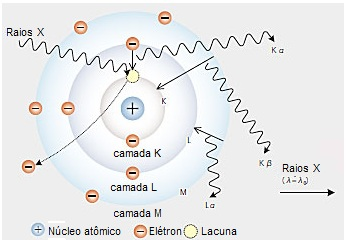
\includegraphics[width=0.5\textwidth]{../inputs/images/shimadzu_atomo.jpg}
  \caption{Shimadzu - Figura que acompanha o manual do XRF-ED \label{fig:shimadzu_atomo}}
   % http://www.shimadzu.com.br/analitica/produtos/elemental/raios_x/eds/images/edx-7000_8000-2.jpg
\end{center}
\end{figure}

O feixe de raios X incidente, produzido por tudo de raios X, fontes radioativas
ou por partículas aceleradas, expulsa os elétrons das camadas mais 
internas $K$ e $L$, produzindo vacâncias. 
Um átomo com vacância é instável e rapidamente elétrons das camadas 
mais externa preenchem as vacâncias estabilizando o átomo.

As transições dos elétrons entre o nível quântico $L$ e
$K$ liberam raios X característicos do átomo em questão. 

Transições da camada $L$ para $K$ são do tipo $K\alpha$, de $M$ para $K$ 
são $K\beta$ e de $M$ para $L$ são $L\alpha$ ou $L\beta$. 
A camada $L$ possue 3 e a camada $M$ 5 subníveis o que
resulta em inúmeras possibilidades de transições, sendo que algumas transições
proibidas. 

A \textit{notação de Siegbahn} permite identificarmos melhor os subníveis
de origen e destino, por exemplo, transição de $M_{IV}$ para $L_{III}$ é uma transição do 
tipo $L\beta_1$ \cite{jenkins1991}, outras possíveis pode ser vista na
figura \ref{fig:siegbahn}. 

\begin{figure}[H]
\begin{center} 
  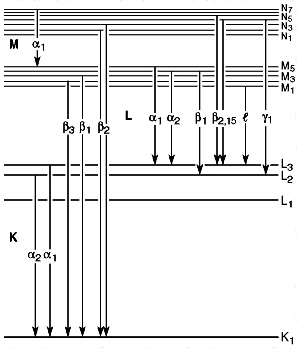
\includegraphics[width=0.5\textwidth]{../inputs/images/Siegbahn.jpg}
  \caption{Transições - artigo \cite{jenkins1991}  \label{fig:siegbahn}}
\end{center}
\end{figure}

Entretanto, há transições com energias são tão próximas 
que são indistinguiveis para os detectores (semicondutores) 
utilizados, sendo assim, neste trabalho vamos chamar apenas de 
transições tipo $K$ e $L$.

%%%%
\subsection{Fluorescência de Raios X por dispersão em energia}

A \textit{Fluorescência de Raios X por dispersão em energia} (\textbf{XRF-ED}).
usa detectores de semicondutores capaz de discriminar energia 
próximas, onde a distinção dos fótons é feita pela amplitude do pulso 
eletrônico produzido no detector, pois os pulsos eletrônicos são
proporcionais às energias dos raios X incidentes. 

O detector mais empregado é o de silício ativado com lítio $Si(Li)$ 
O sistema eletrônico do equipamento armazena o pulso em um multicanal.

Características da \textbf{XRF-ED} do IAG-USP e opções usadas nessa pesquisa:
\begin{itemize}
  \item marca e modelo: EDX-720/800HS
  \item tipo de tubo de raios x: ródio Rh
  \item tensão aplicada no tubo: 50 KV 
  \item detector: Si(Li)
  \item multicanal: 2048 canais
  \item filtro: Al
  \item corrente: 1000 $\mu A$
  \item energia: 0 - 20 $KeV$ 
  \item tempo morto médio: 13\%
  \item tempo de análise: 18 minutos.
\end{itemize}

\begin{figure}[H]
\begin{center}
  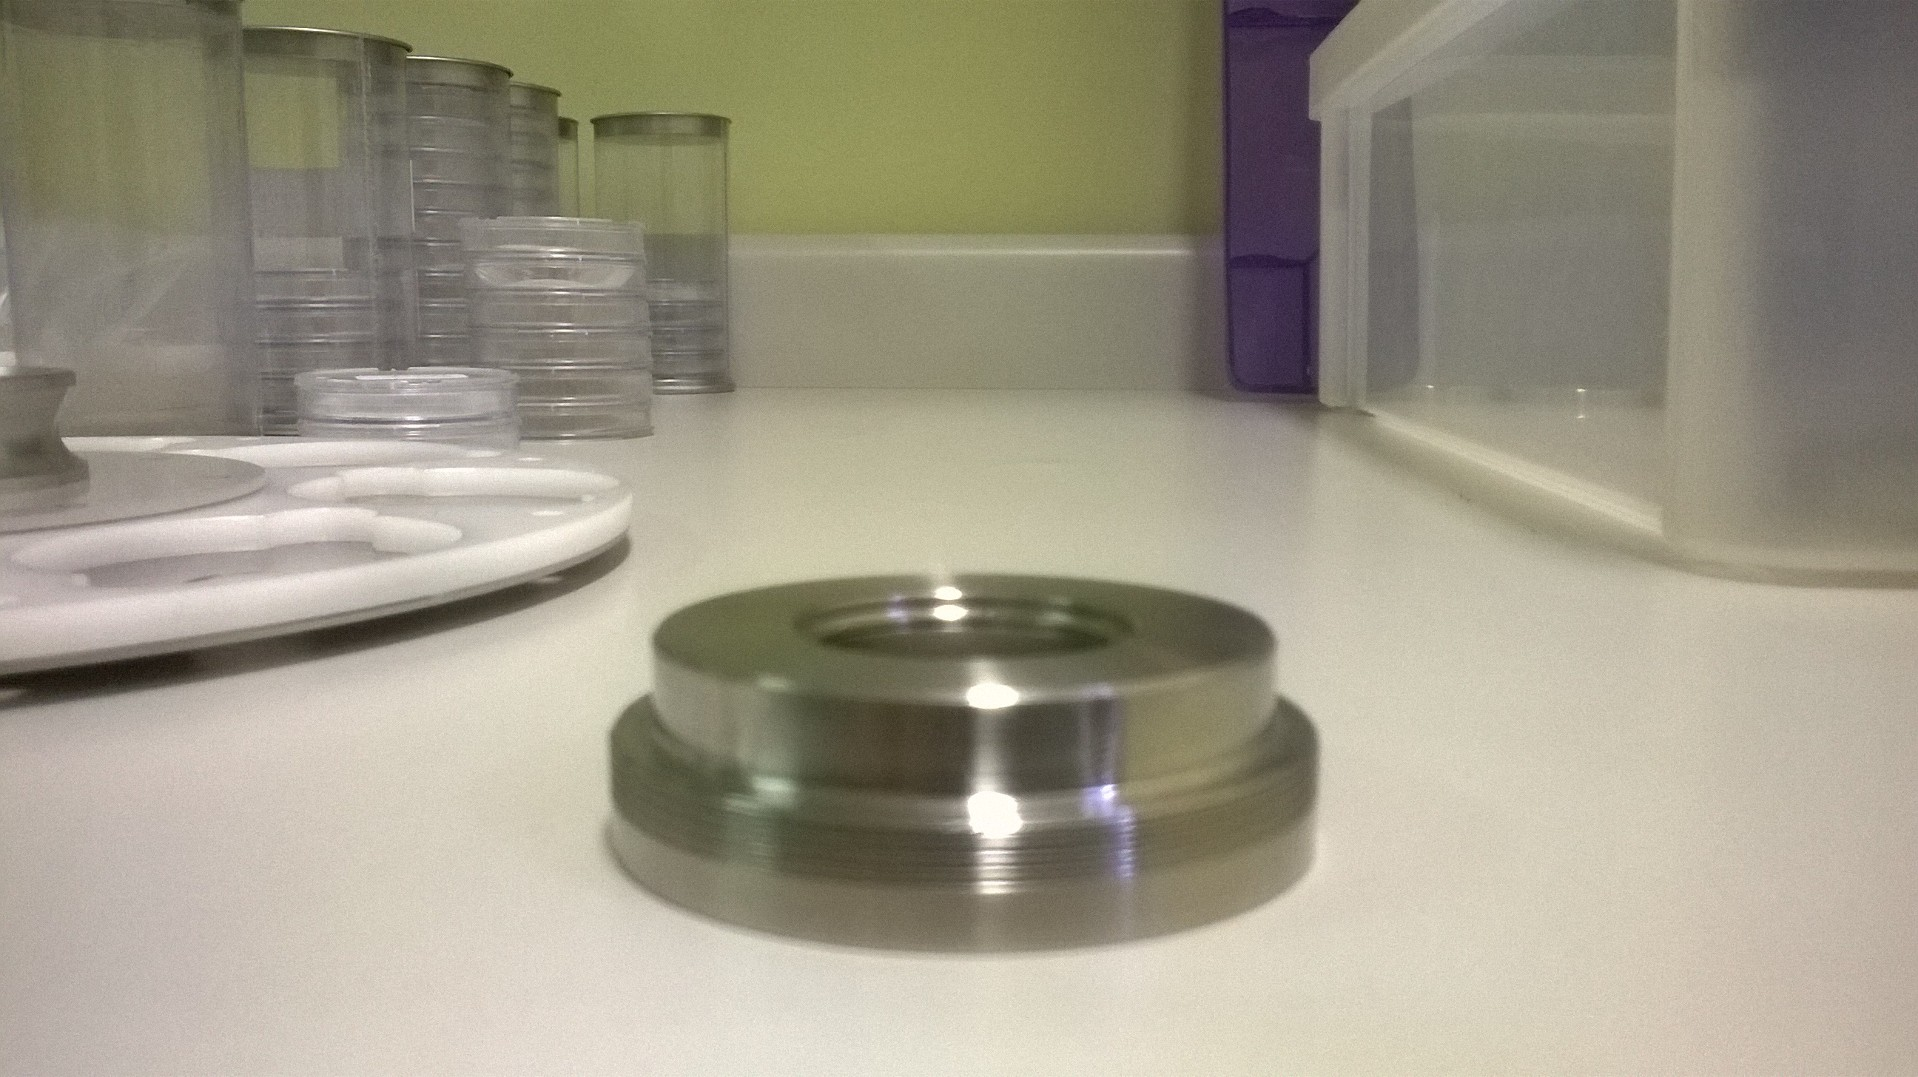
\includegraphics[scale=0.4]{../inputs/images/suporte8.jpg}
  \caption{Suporte 8- \label{fig:suporte8}}
\end{center}
\end{figure}

\begin{figure}[H]
\begin{center}
  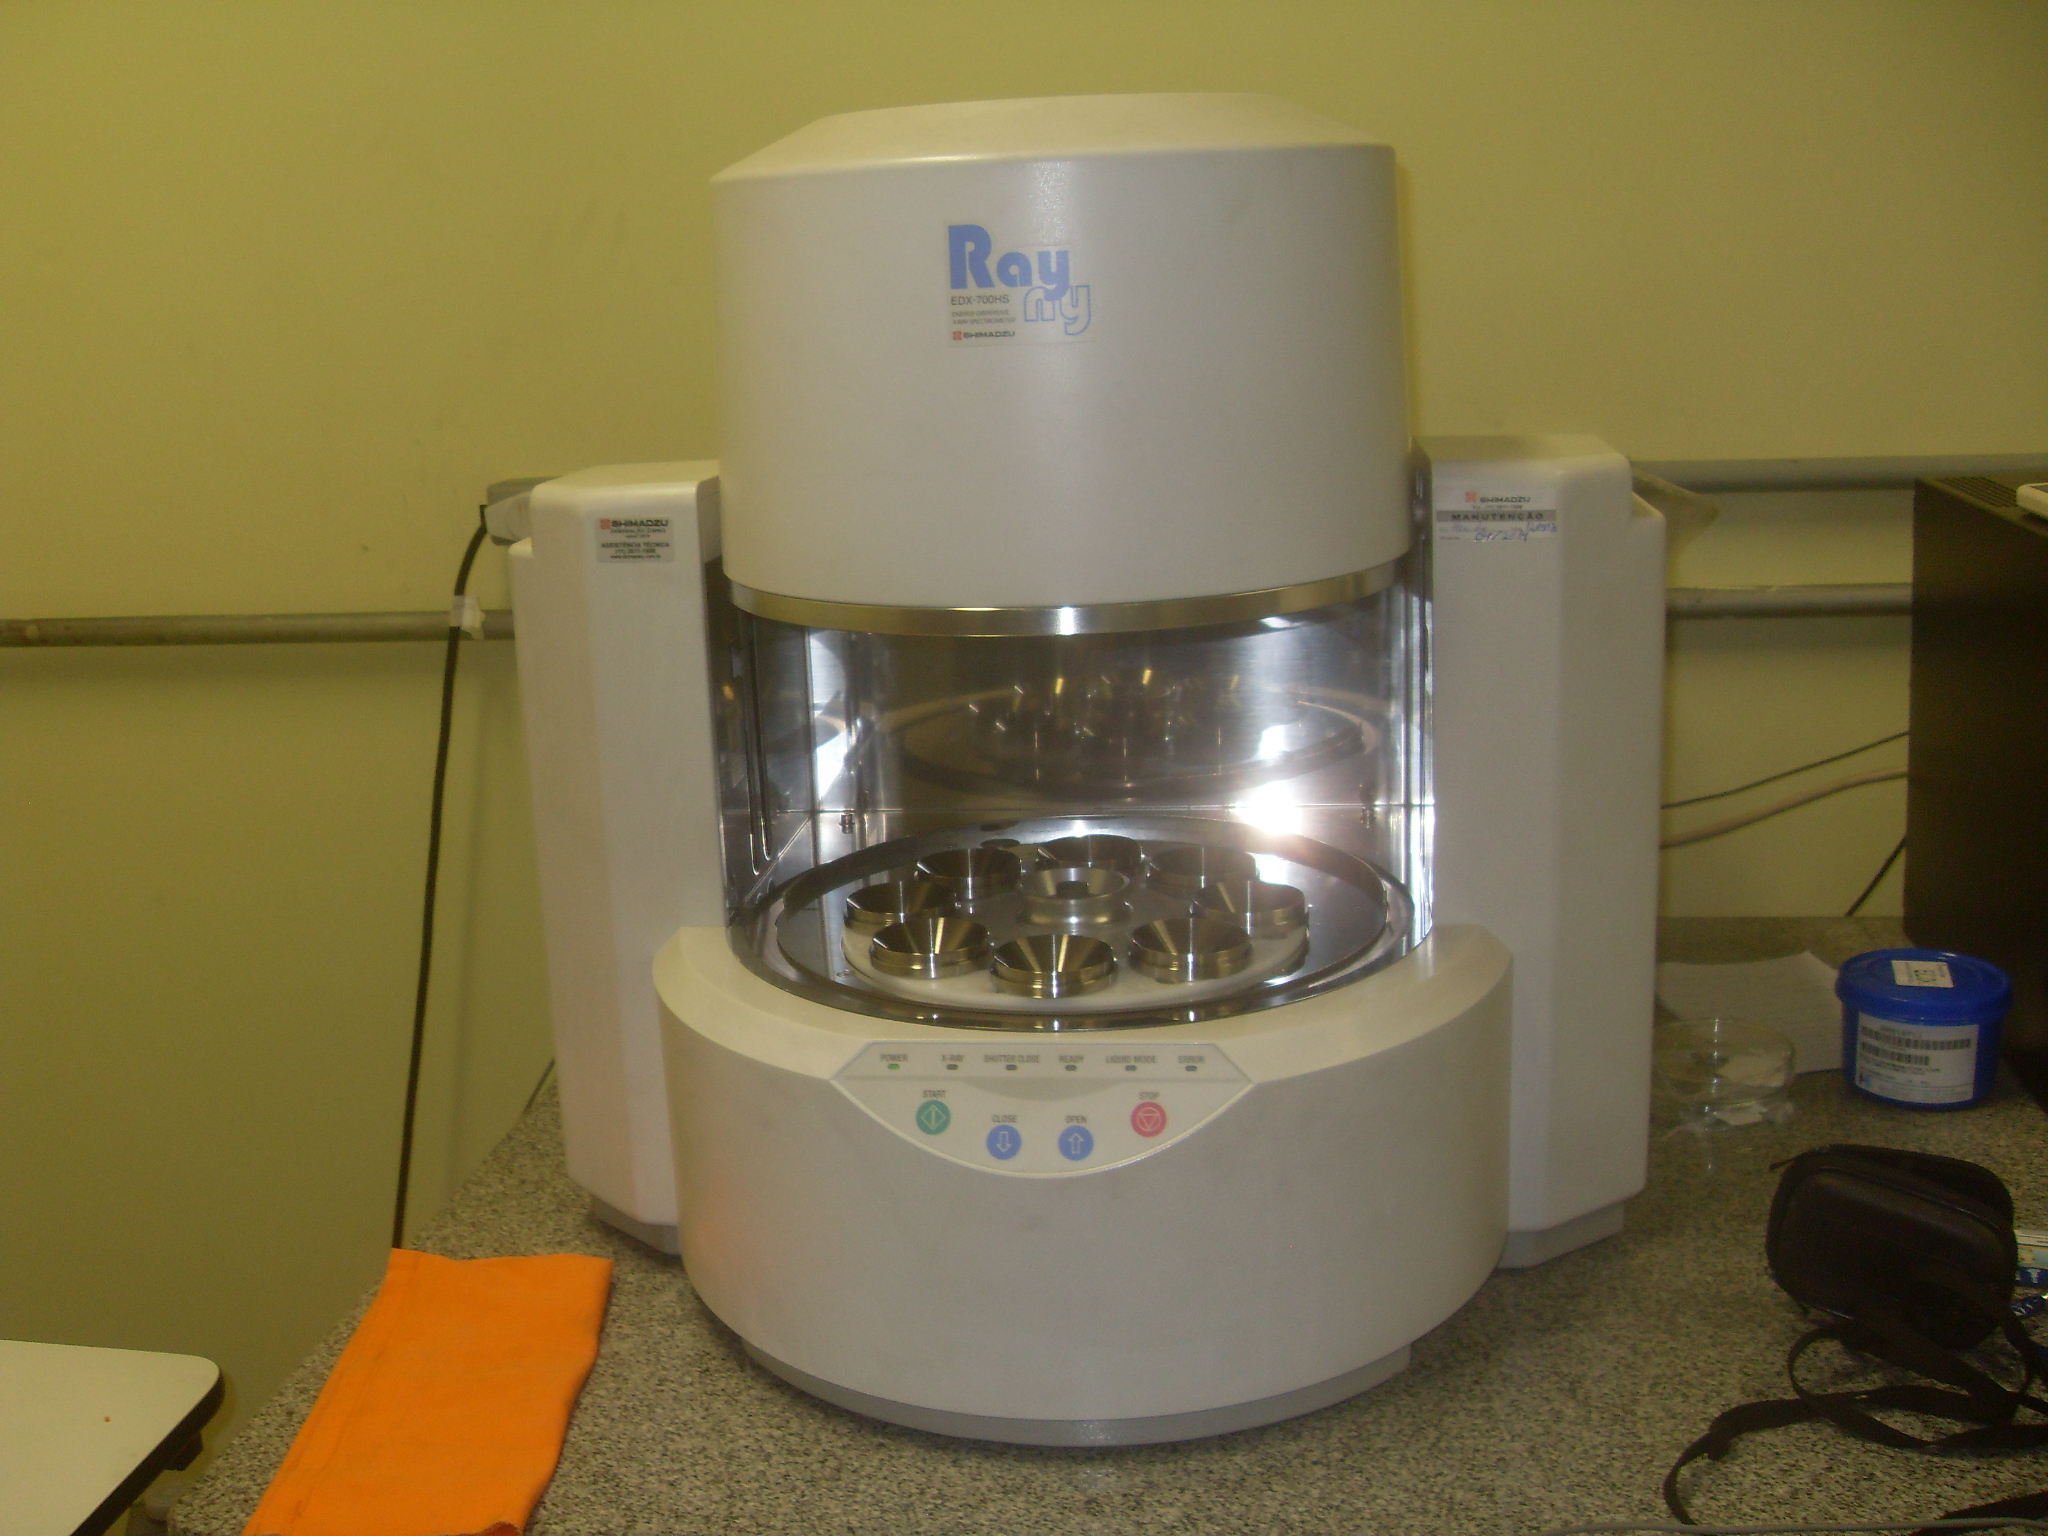
\includegraphics[scale=0.4]{../inputs/images/xrf-ed-IAG-USP.jpg}
  \caption{\textbf{XRF-ED} do IAG-USP - \label{fig:xrfed_iag}}
\end{center}
\end{figure}



%TODO: Colocar espectro plot 

A análise dos espectros obtidos por esses métodos foram feitas no software WinQxas (IAEA, 2002).





E a figura \ref{fig:xrfed_iag} ...

\begin{figure}[H]
\begin{center}
  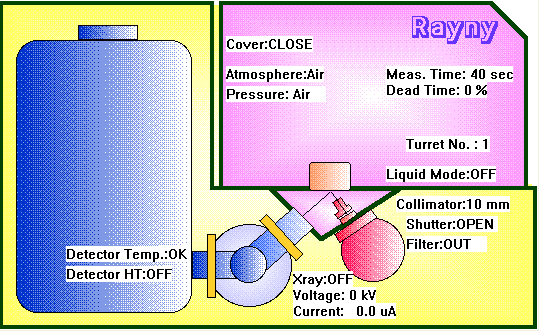
\includegraphics[scale=0.4]{../inputs/images/edx_iag_monitor.png}
  \caption{Fluorescência de Raios X por dispersão em energia do IAG USP - \label{fig:xrfed_software}}
\end{center}
\end{figure}

%%%%
\subsection{Calibração}

O método \textit{PIXE (Particle Induced X-Ray Emission)}, 
também comumente usado em análises ambientais, usa feixe de íons 
(prótons ou alfas) para excitação dos átomos das amostras.

\begin{figure}[H]
\begin{center} 
  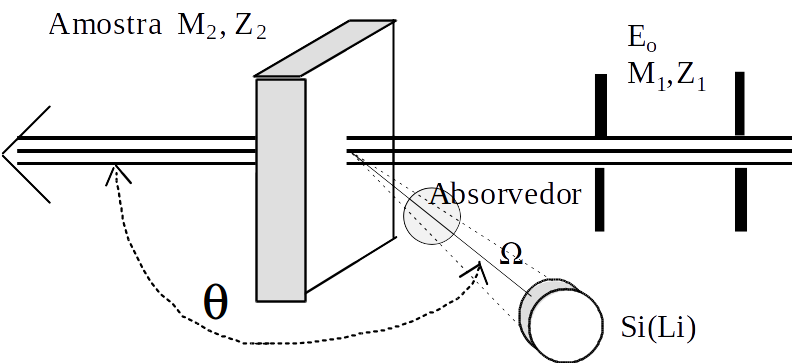
\includegraphics[width=0.8\textwidth]{../inputs/images/arranjopixe.png}
  \caption{Arranjo experimental básico para análise de método PIXE 
           \cite{tabacniks2000} \label{fig:arranjopixe}}
\end{center}
\end{figure}

Baseado no arranjo experimental da figura \ref{fig:arranjopixe} e
considerando o filtro fino (alguns $\mu m$),
\cite{tabacniks2000} chega na equação \ref{eq:npixe} para quantidade de Raios X
contadas no detector. 

\begin{equation}
  \label{eq:npixe}
  N(Z) = \frac{\Omega}{4\pi} \sigma \zeta T t_z \frac{Q}{qe}
\end{equation}

Sendo que, o número de raios X detectados $N(Z)$ é proporcional à 
densidade (massa ou átomos por área) $t_Z$ e a carga coletada $Q$.
$Z$ é espécie química, $\zeta$ é a eficiência do detector, 
$\sigma_x$ é a secção de choque, $\Omega$ é o ângulo sólido, 
$T$ é a transmitância para raios-X em caso de uso de absorvedores 
(colocados entre a amostra e o detector), $q$ é o estado de carga da 
partícula incidente e $e$ é a carga do elétron \cite{tabacniks2000}.

Para resolver a equação \ref{eq:npixe}, parâmetros do arranjo experimental
($\Omega$, $\sigma$, $\zeta$ e $T$) deveriam ser conhecidos. 

Na prática, é mais comum é irradiar alvos de calibração com $t_z$ conhecidos,
e encontrar uma variável única proporcional aos parâmetros do arranjo experimental.
Da-se o nome de fator de resposta $R(Z)$ a essa variável.

Assim, a equação \ref{eq:npixe} é simplificada pela equação \ref{eq:contagem}.

\begin{equation}
  \label{eq:contagem}
  N(Z) = R(Z) I\Delta t \frac{m(Z)}{a}
\end{equation}

$R(Z)$ é o fator de resposta, $I\Delta t$ é a carga efetiva expressa
em termos da corrente e do tempo efetivo de análise e a 
a massa $m(Z)$ e a área $a$ representam a densidade $t_z$. 

Alvos de calibração podem ser comprados ou produzidos, dependendo da 
precisão desejada. Isolando-se $R(Z)$, obtemos a \ref{eq:fator_de_resposta}.

\begin{equation}
  \label{eq:fator_de_resposta}
  R(Z) = \frac{N(Z) a}{m(Z)I \Delta t}
\end{equation}

Assim, para cada elemento que se tem alvo padrão, pode-se calcular $R(Z)$,
pois, nos alvos padrões a densidade ($m(Z)/a$) é conhecida e $N(Z)$, $I \Delta t$ são medidos. 

Conhecendo-se o fator de resposta $R(Z)$, pode-se calcular a massa $m(Z)$ da espécie química
desejada pela equação \ref{eq:xrfedmassa}, que nada mais é que o isolamento de $m(Z)$ na 
\ref{eq:contagem}. 

\begin{equation}
  \label{eq:xrfedmassa}
  m(Z) = \frac{N(Z) a}{ R(Z)I \Delta t}
\end{equation}

Entretanto, para cada espécie química de interesse, seria necessário 
o alvo de calibração correspondente.

Nem sempre é possível adiquirir alvos de calibração para todos elementos
químicos e a incerteza garantida pelos fabricantes (exemplo \textit{MICROMATTER}) é de
5\%. 

Fazendo-se um ajuste polinomial com os $R(Z)$ disponíveis, mostrou-se uma estratégia 
que contornou a falta de filtros de calibração para algumas espécies, abordada melhor
no capítulo de Resultados. 

O ajuste polinomial ainda proporcionou incertezas menores que 5\% para todas espécies, 
inclusive para aquelas que tínhamos os alvos de calibrações.

%%%%
\subsection{Estimativa do erro}

Para a estimativa do erro do ajuste, utilizou-se o 
\textit{Ajuste dos Mínimos Quadrados Matricial} \cite{helene2006}.

Dada uma variável $Y_i$ com relação polinomial com $X_i$ 
\begin{equation}
  \label{eq:polinomio}
  \begin{split}
    y_1 = a + b x_1 + c{x_1}^2 + d{x_1}^3 + ...\\
    y_2 = a + b x_2 + c{x_2}^2 + d{x_2}^3 + ... \\
    ...
  \end{split}
\end{equation}

A representação matricial da equação \ref{eq:polinomio}:
\begin{equation}
  \label{eq:polinomioMatriz}
  [Y] = [A][X]
\end{equation}

Os coeficientes ajustados $[Ã]$ são dados pela equação \ref{eq:coeficientesajustados},
que depende da matriz de covariância dos coeficientes $[V_{Ã}]$, 
dada pela equação \ref{eq:matrizcovariancia}.

\begin{equation}
  \label{eq:coeficientesajustados}
  [Ã] = [V_{Ã}] ([X]^T {[V_Y]}^{-1} [Y])
\end{equation}

\begin{equation}
  \label{eq:matrizcovariancia}
  [V_{Ã}] = ([X]^T [V_Y]^{-1} [X])^{-1}
\end{equation}

Com o coeficientes ajustados $[Ã]$ pode-se calcular os $[\tilde{Y}]$ ajustado \ref{eq:polinomioajustado}.
\begin{equation}
  \label{eq:polinomioajustado}
  [\tilde{Y}] = [Ã][X]
\end{equation}

Por fim, a incerteza é dada pela diagonal da matriz de covariância de $[\tilde{Y}]$, 
$[V_{\tilde{Y}}]$ em \ref{eq:matrizcovarianciaY}.

\begin{equation}
  \label{eq:matrizcovarianciaY}
  [V_{\tilde{Y}}] = [X] [V_{Ã}]^{-1} [X]^{-1}
\end{equation}

Adaptando-se para nosso contexto, $[Y]$ será os fatores de respostas $[R]$,
e $[X]$ os números atômicos $[Z]$.

%%%%
\subsection{Limite de Detecção}

Densidade mínima para haver detecção da espécie. % como determina para XRF?

Amostra espessas apresentam o efeito matriz, ou seja, interações dos 
raios X característicos com os elementos da amostras, causando 
absorção do raios X ou mesmo reforço de raios X.

%%%%
\subsection{Fontes de erro no branco}

Quando se tem N alvos brancos, a concentração do elemento 
considerado será a média sobre os N dados e o desvip padrão $\sigma_p$.

Mas quando N<10 é pequeno, precisa haver um fator de correção conforme tabela.

\begin{table}[H]
\centering
\caption{My caption}
\label{my-label}
\begin{tabular}{ll}
N  & Fator \\
2  & 1,84  \\
3  & 1,32  \\
4  & 1,20  \\
5  & 1,14  \\
6  & 1,12  \\
7  & 1,11  \\
8  & 1,09  \\
9  & 1,08  \\
10 & 1,06  \\
20 & 1,03 
\end{tabular}
\end{table}

%Já o erro da integração do espectro é calculado pelo erro na integração de cada espectro de branco e, obviamente, tem que ser calculado sem branco, só com o fator de resposta (ou seja, a rotina que calcula a concentração tem que ser igual para o alvo comum e para o branco; mas o alvo comum tem que ter uma complementação no cálculo para subtrair o branco e adicionar o erro, devido ao branco). Havendo N alvos brancos, com erro  i de integração para cada um deles, o erro transferido para a média deve ser:





